% Options for packages loaded elsewhere
\PassOptionsToPackage{unicode}{hyperref}
\PassOptionsToPackage{hyphens}{url}
%
\documentclass[
]{article}
\usepackage{amsmath,amssymb}
\usepackage{iftex}
\ifPDFTeX
  \usepackage[T1]{fontenc}
  \usepackage[utf8]{inputenc}
  \usepackage{textcomp} % provide euro and other symbols
\else % if luatex or xetex
  \usepackage{unicode-math} % this also loads fontspec
  \defaultfontfeatures{Scale=MatchLowercase}
  \defaultfontfeatures[\rmfamily]{Ligatures=TeX,Scale=1}
\fi
\usepackage{lmodern}
\ifPDFTeX\else
  % xetex/luatex font selection
\fi
% Use upquote if available, for straight quotes in verbatim environments
\IfFileExists{upquote.sty}{\usepackage{upquote}}{}
\IfFileExists{microtype.sty}{% use microtype if available
  \usepackage[]{microtype}
  \UseMicrotypeSet[protrusion]{basicmath} % disable protrusion for tt fonts
}{}
\makeatletter
\@ifundefined{KOMAClassName}{% if non-KOMA class
  \IfFileExists{parskip.sty}{%
    \usepackage{parskip}
  }{% else
    \setlength{\parindent}{0pt}
    \setlength{\parskip}{6pt plus 2pt minus 1pt}}
}{% if KOMA class
  \KOMAoptions{parskip=half}}
\makeatother
\usepackage{xcolor}
\usepackage[margin=1in]{geometry}
\usepackage{longtable,booktabs,array}
\usepackage{calc} % for calculating minipage widths
% Correct order of tables after \paragraph or \subparagraph
\usepackage{etoolbox}
\makeatletter
\patchcmd\longtable{\par}{\if@noskipsec\mbox{}\fi\par}{}{}
\makeatother
% Allow footnotes in longtable head/foot
\IfFileExists{footnotehyper.sty}{\usepackage{footnotehyper}}{\usepackage{footnote}}
\makesavenoteenv{longtable}
\usepackage{graphicx}
\makeatletter
\def\maxwidth{\ifdim\Gin@nat@width>\linewidth\linewidth\else\Gin@nat@width\fi}
\def\maxheight{\ifdim\Gin@nat@height>\textheight\textheight\else\Gin@nat@height\fi}
\makeatother
% Scale images if necessary, so that they will not overflow the page
% margins by default, and it is still possible to overwrite the defaults
% using explicit options in \includegraphics[width, height, ...]{}
\setkeys{Gin}{width=\maxwidth,height=\maxheight,keepaspectratio}
% Set default figure placement to htbp
\makeatletter
\def\fps@figure{htbp}
\makeatother
\setlength{\emergencystretch}{3em} % prevent overfull lines
\providecommand{\tightlist}{%
  \setlength{\itemsep}{0pt}\setlength{\parskip}{0pt}}
\setcounter{secnumdepth}{-\maxdimen} % remove section numbering
\ifLuaTeX
  \usepackage{selnolig}  % disable illegal ligatures
\fi
\IfFileExists{bookmark.sty}{\usepackage{bookmark}}{\usepackage{hyperref}}
\IfFileExists{xurl.sty}{\usepackage{xurl}}{} % add URL line breaks if available
\urlstyle{same}
\hypersetup{
  pdftitle={Health Analysis},
  pdfauthor={Lynn Ajema},
  hidelinks,
  pdfcreator={LaTeX via pandoc}}

\title{Health Analysis}
\author{Lynn Ajema}
\date{2023-09-26}

\begin{document}
\maketitle

\begin{verbatim}
 [1] "~$Dataset.xlsx"        "County.dbf"            "County.prj"           
 [4] "County.sbn"            "County.sbx"            "County.shp"           
 [7] "County.shp.xml"        "County.shx"            "Dataset.xlsx"         
[10] "Health-Analysis.html"  "Health-Analysis.Rmd"   "Health-Analysis_files"
[13] "Health Analysis.Rmd"   "kenya_map.html"        "kenya_map.png"        
\end{verbatim}

\begin{verbatim}
# A tibble: 47 x 29
   Country COUNTY    Rural_ppn Urban_ppn `Total Population` `Urban/Total` Status
   <chr>   <chr>         <dbl>     <dbl>              <dbl>         <dbl> <chr> 
 1 Kenya   Baringo      591474     75289             666763        0.113  Rural 
 2 Kenya   Bomet        847718     27971             875689        0.0319 Rural 
 3 Kenya   Bungoma     1480458    190112            1670570        0.114  Rural 
 4 Kenya   Busia        779928    113753             893681        0.127  Rural 
 5 Kenya   Keiyo-Ma~    433901     20579             454480        0.0453 Rural 
 6 Kenya   Embu         532675     75924             608599        0.125  Rural 
 7 Kenya   Garissa      630463    210890             841353        0.251  Rural 
 8 Kenya   Homa Bay    1018871    113079            1131950        0.0999 Rural 
 9 Kenya   Isiolo       142333    125669             268002        0.469  Urban 
10 Kenya   Kajiado      495218    622622            1117840        0.557  Urban 
# i 37 more rows
# i 22 more variables: Surface_area <dbl>,
#   `PPn_density(people per sq. km)` <dbl>, Subcounties <dbl>,
#   Constituencies <dbl>, Wards <dbl>,
#   `Contribution of Agriculture forestry and fishing %` <dbl>,
#   `Contribution to GDP %` <dbl>, Health_LV5 <dbl>, Health_LV4 <dbl>,
#   Health_LV3 <dbl>, Health_LV2 <dbl>, `Bed density per 10000 ppn` <dbl>, ...
\end{verbatim}

\begin{verbatim}
## Reading layer `County' from data source `D:\DTE-Datathon\LYNN ANALYSIS\County.shp' using driver `ESRI Shapefile'
## Simple feature collection with 47 features and 8 fields
## Geometry type: MULTIPOLYGON
## Dimension:     XY
## Bounding box:  xmin: 33.91182 ymin: -4.702271 xmax: 41.90626 ymax: 5.430648
## Geodetic CRS:  WGS 84
\end{verbatim}

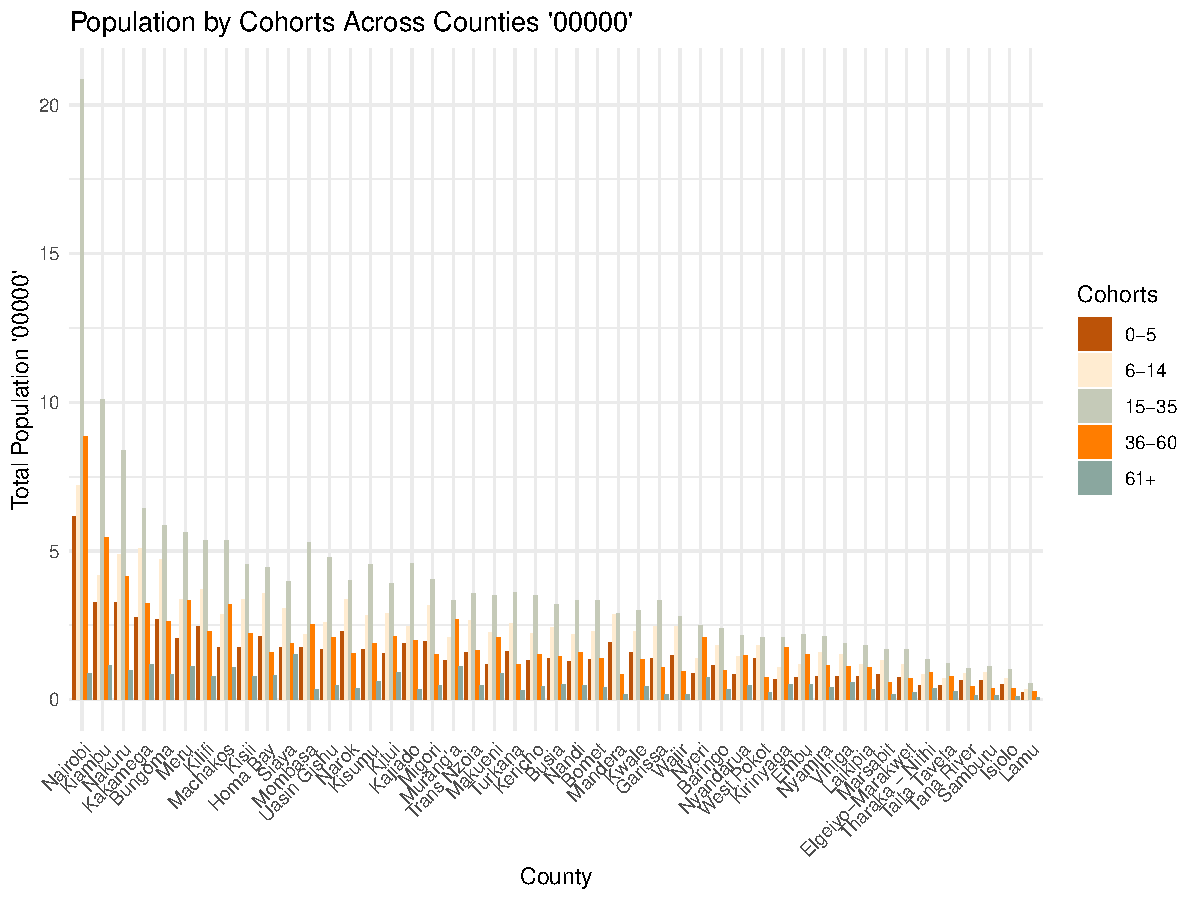
\includegraphics{Health-Analysis_files/figure-latex/unnamed-chunk-4-1.png}

\#Health Analysis \#\# How many countys have level 5/6 hospitals

\begin{longtable}[]{@{}lr@{}}
\caption{Count of Level 5/6 Hospitals by County}\tabularnewline
\toprule\noalign{}
COUNTY & Health\_LV5 \\
\midrule\noalign{}
\endfirsthead
\toprule\noalign{}
COUNTY & Health\_LV5 \\
\midrule\noalign{}
\endhead
\bottomrule\noalign{}
\endlastfoot
Embu & 1 \\
Garissa & 1 \\
Homa Bay & 1 \\
Kakamega & 1 \\
Kiambu & 3 \\
Kisii & 2 \\
Kisumu & 1 \\
Machakos & 1 \\
Mandera & 1 \\
Meru & 1 \\
Mombasa & 1 \\
Nairobi & 7 \\
Nakuru & 1 \\
Nandi & 1 \\
Nyeri & 2 \\
Trans Nzoia & 1 \\
Uasin Gishu & 1 \\
\end{longtable}

\hypertarget{bar-chart-showing-level-4-hospital-distribution-among-rural-counties}{%
\subsection{Bar chart showing Level 4 hospital distribution among Rural
counties}\label{bar-chart-showing-level-4-hospital-distribution-among-rural-counties}}

\#\#Bar chart showing Level 4 hospital distribution in Urban counties

\#\#Bar chart showing Level 3 hospitals distribution by Rural counties

\#\#Bar chart showing ditribution of level 3 Hospitals in Urban counties

\#\#Bar chart showing Level 2 Hospitals distribution by Rural county

\#\#Bar chart showing Level 2 hospital distribution by Urban counties

\#\#Bar chart showing hospital bed density per 10000 population by Rural
Counties

\#\#Bar chart showing hospital bed density per 10000 population by Urban
counties

\#\#Bar chart showing Health worker per 10000 ppn by Rural county

\#\#Bar chart showing Health worker per 10000 ppn by Urban county

\includegraphics{Health-Analysis_files/figure-latex/unnamed-chunk-16-1.pdf}

\includegraphics{Health-Analysis_files/figure-latex/unnamed-chunk-17-1.pdf}

\includegraphics{Health-Analysis_files/figure-latex/unnamed-chunk-18-1.pdf}

\includegraphics{Health-Analysis_files/figure-latex/unnamed-chunk-19-1.pdf}

\includegraphics{Health-Analysis_files/figure-latex/unnamed-chunk-20-1.pdf}

\end{document}
